\documentclass[11pt]{exam}
\usepackage[margin=1in]{geometry}
\pagestyle{plain}
\usepackage{amsmath,amsfonts,amssymb,amsthm,enumerate}
\usepackage{multicol}
\usepackage[]{graphicx}
\usepackage{hyperref}
\usepackage{tikz}
\usepackage{pgfplots}
\usepackage{subfigure}
\usepackage[final]{pdfpages}

\addtolength{\footskip}{2\baselineskip} % to lower the page numbers
\title{\vspace{-0.5in} Math 115 \\ Worksheet Section 4.4}
\date{}


% \theoremstyle{definition}
% \newtheorem{problem}{Problem}
\renewcommand{\questionlabel}{\textbf{Problem~\thequestion.}}
%\printanswers

\begin{document}
\maketitle
\vspace{-0.75in}
\begin{questions}
  \question Consider the family of functions $\quad f(x) = e^{-(x-a)^2/b}, \; \text{for} \; b>0$.

    Find
    \begin{enumerate}
    \item \(f(0)\),
    \item $\displaystyle \lim_{x\to\infty}f(x)$,
    \item $\displaystyle \lim_{x\to-\infty} f(x)$, and
    \item any local maxima and minima.
    \item Sketch \(f\).
    \end{enumerate}
    \begin{solution}
      \begin{enumerate}
      \item \(f(0) = e^{-a^2/b}\)
      \item \(\lim_{x \to \infty} f(x) = 0\)
      \item \(\lim_{x \to -\infty} f(x) = 0\)
      \item \(f’(x) = -\frac{2}{b}(x-a) e^{-(x-a)^2/b}\) which is
        defined everywhere and is equal to zero only at \(x=a\).
        For \(x < a\), \(f’(x) = -(-)(+) = +\) and for \(x > a\),
        \(f’(x) = -(+)(+) = -\). So, we get sign line \\
        \begin{tikzpicture}
\node at (-0.5,0) {\(f'\)};
\draw (0,0)--(4,0);
\node at (1,.2) {+};
\node at (2,-.4) {$0$};
\node at (3,.2) {\(-\)};
\end{tikzpicture}
Since \(x=0\) is the only critical point and \(f(0) > 0\), \(x=0\) must
be a global max.
      \item  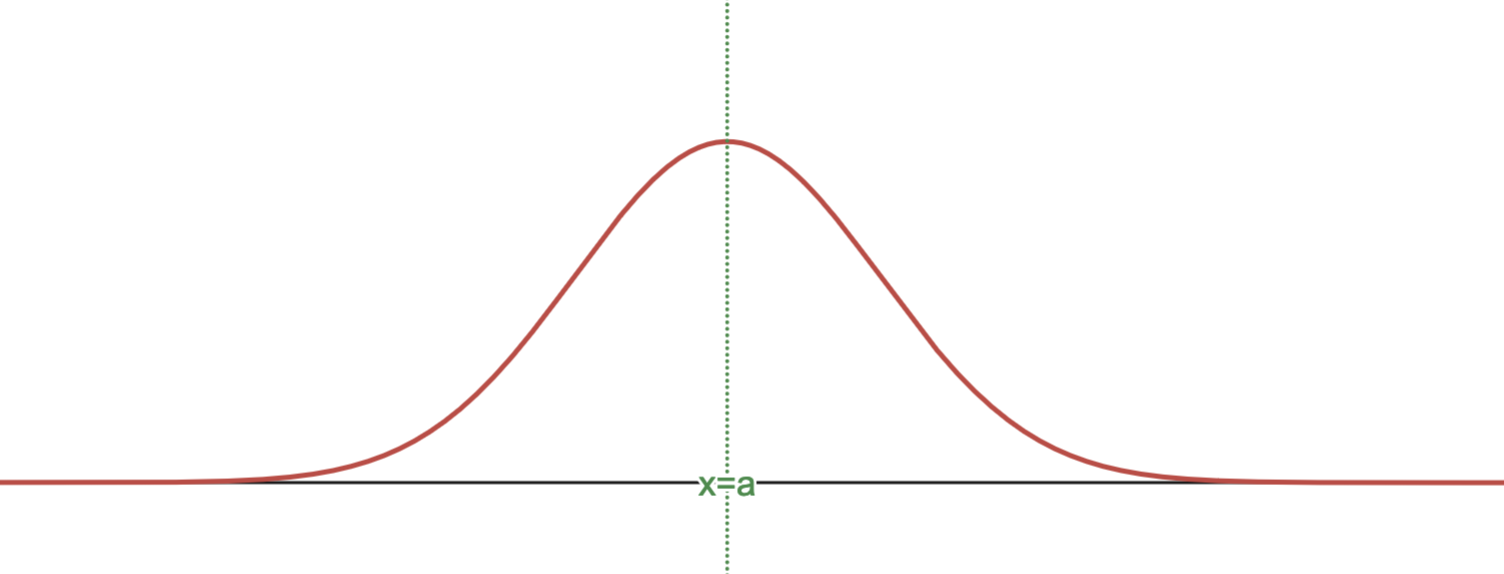
\includegraphics[width=3.3in]{bell-curve.png}
      \end{enumerate}
    \end{solution}
    \vspace{1in}
   \question The graphs of $f(x)=xe^{-ax}$ for $a=1,2,3$ are below.  Find the critical point(s) of $f$, and use this information to identify which graph is which.

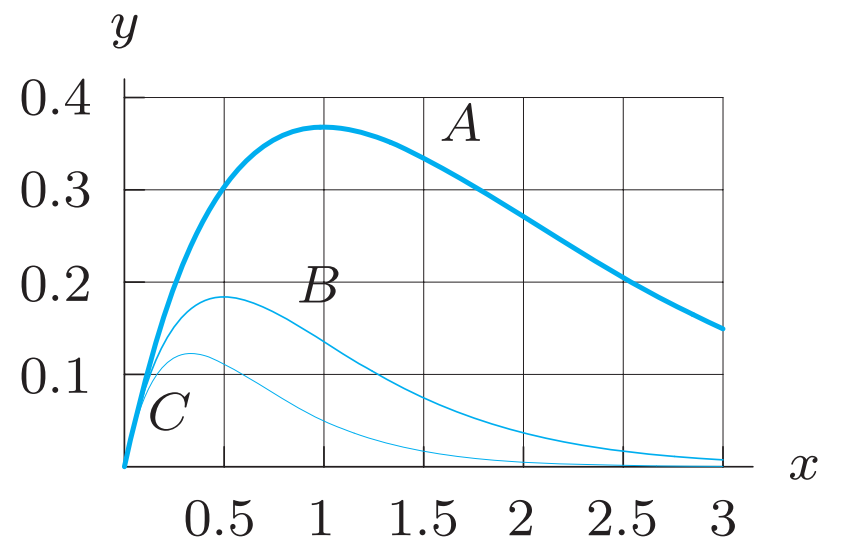
\includegraphics[width=2.5in]{graph.png} 
\begin{solution}
  \(f’(x) = -axe^{-ax} + e^{-ax} = (1-ax)e^{-ax}\) so \(f’(x) = 0\) at
  \(x = \frac{1}{a}\).
  \begin{enumerate}
  \item \(a=1 \implies\) critical point at \(x=1\), so we get graph \(A\).
  \item \(a=2 \implies\) critical point at \(x=1/2\), so we get graph \(B\).
  \item \(a=3 \implies\) critical point at \(x=1/3\), so we get graph \(C\).
  \end{enumerate}
\end{solution}
   \question  Find a formula for a function of the form $y=ae^{-x} + bx$ with a global minimum at $(1,2)$.  Make sure you justify why $(1,2)$ is a \textbf{global} minimum for your function, not just a local minimum.
     \begin{solution}
       Note \(y’ = -ae^{-x}+b\) and a global minimum at \((1,2)\)
       means \(-ae^{-1}+b = 0\). Since \((1,2)\) is a point on the
       graph, we also have \(2 = ae^{-1}+b\). Solving these two
       equations, we get \(b = 1\) and \(a=e^{-1}\).
       We verify that \((1,2)\) is a global minimum since \(\lim_{x
         \to \infty} y = \infty\) since \(bx\) will dominate
       \(ae^{-x}\) and \(\lim_{x \to -\infty} y = \infty\) since
       \(ae^{-x}\) goes to infinity and will dominate \(bx\) in the
       negative direction.
     \end{solution}
\vspace{1in}
  \question  Find a formula for a cubic polynomial with a critical point at $x=2$, an inflection point at $(1,4)$, and a leading coefficient of 1. 
    \begin{solution}
      A cubic polynomial is of the form \(f(x) = ax^3+bx^2+cx+d\) for
      real numbers \(a,b,c,d\).
      We are given that \(a=1\), \(f(1) = 4\), \(f'(2) = 0\) since \(x=2\) is a
      critical point, and \(f''(1) = 0\) since \((1,4)\) is an
      inflection point. Thus,
      \[
        f'(x) = 3x^2+2bx+c \quad f''(x) = 6x + 2b \,.
      \]
      Then, we can use our various given equations to solve for
      \(b,c,d\).
      \[
        0 = f''(1) = 6+2b \implies b = -3
      \]
      \[
        0 = f'(2) = 3 \cdot 2^2 + 2 \cdot (-3) \cdot 2 + c \implies c=0
      \]
      \[
        4 = f(1) = 1^3-3 \cdot 1^2 - 0 \cdot 1 + d \implies d = 6
      \]
      Thus, we get \(f(x) = x^3-3x^2+6\).
    \end{solution}
    \pagebreak
    \ifprintanswers 
    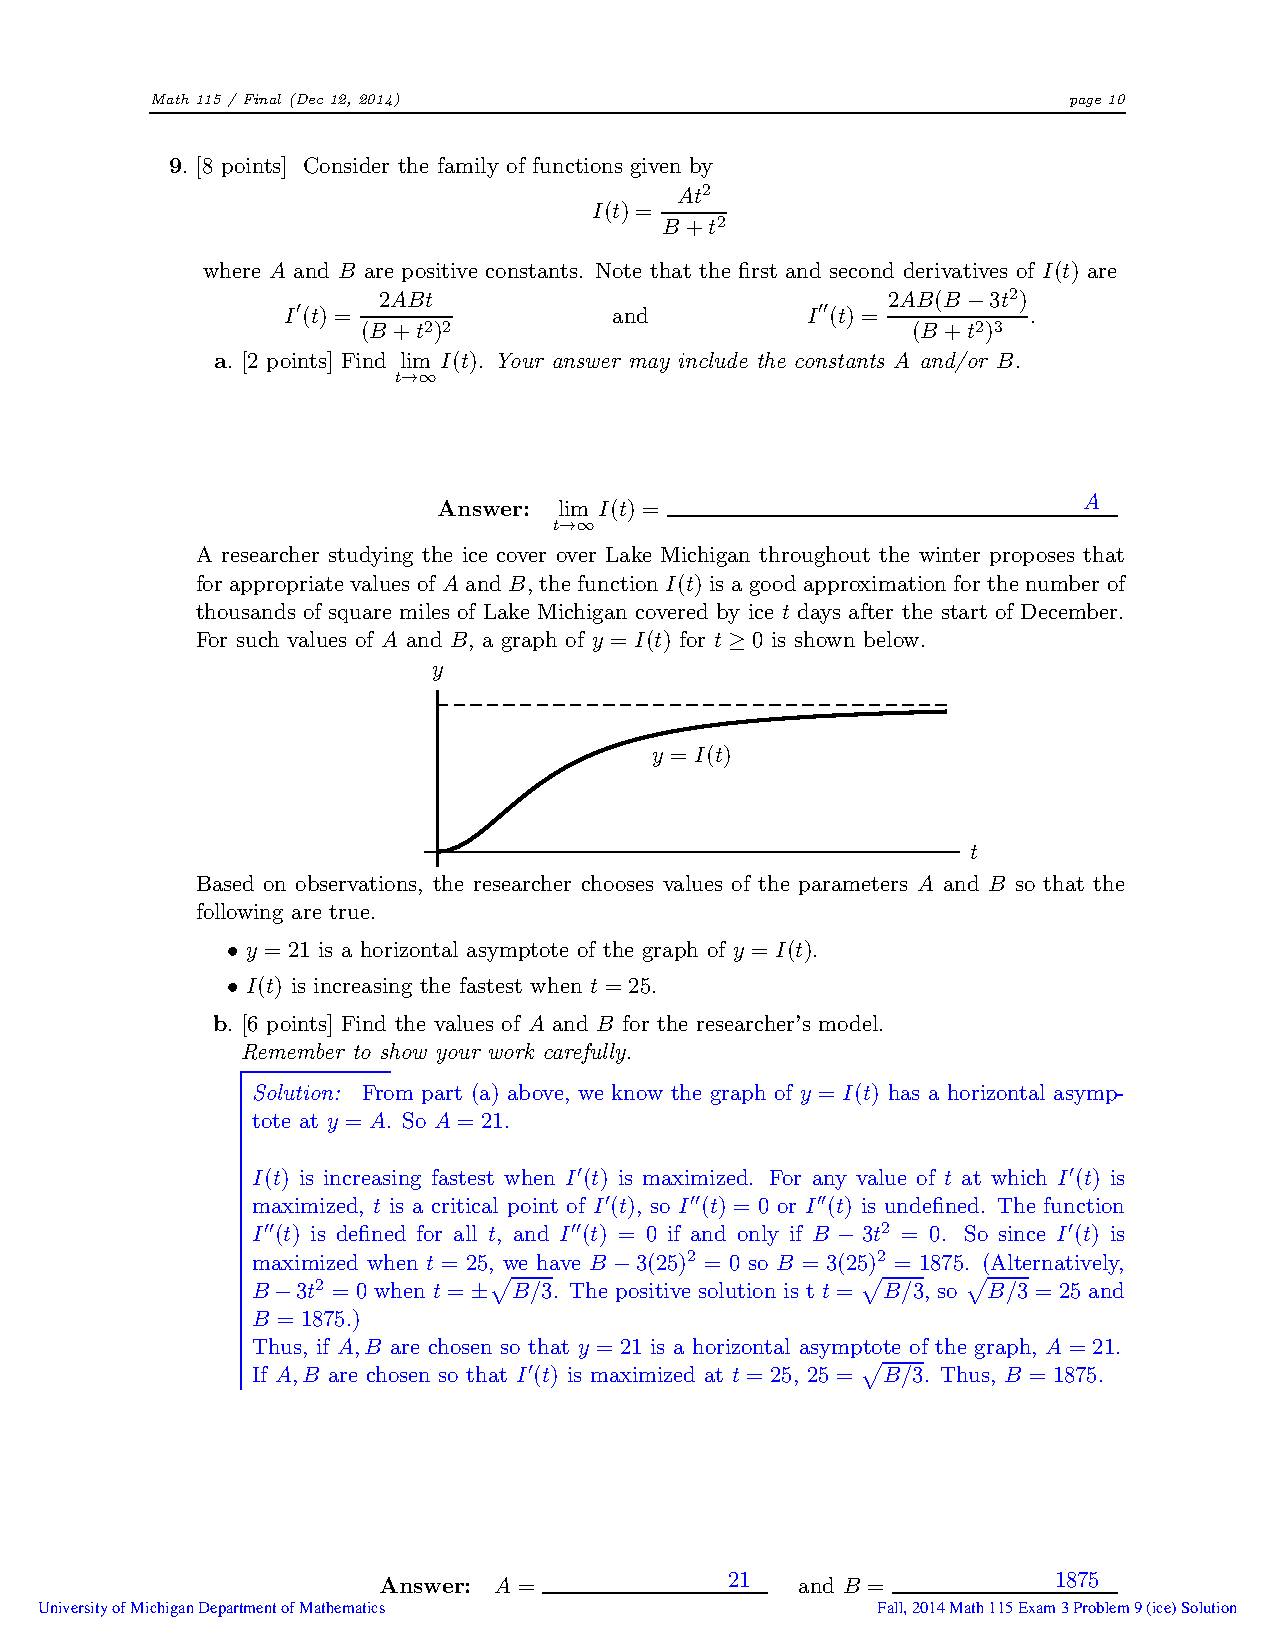
\includepdf[pages=-,pagecommand={}]{s9.pdf}
    \else
    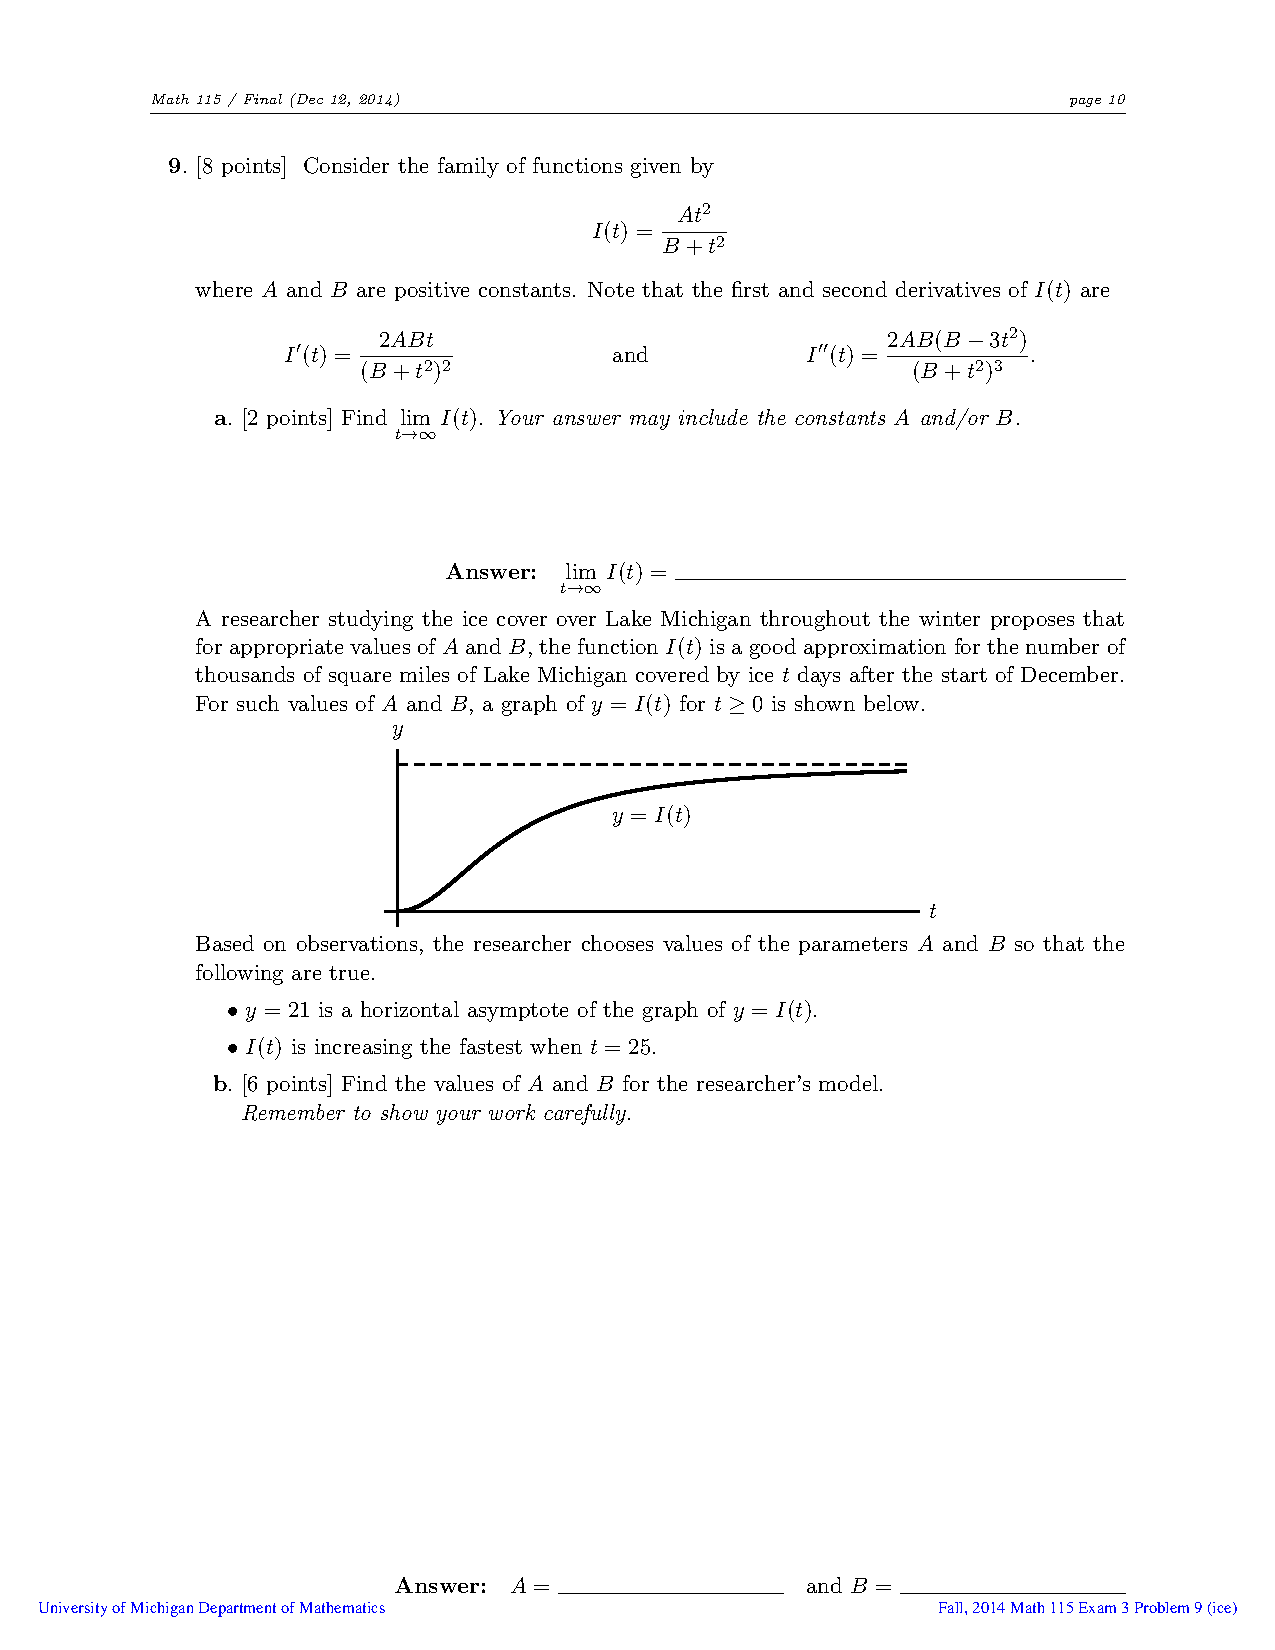
\includepdf[pages=-,pagecommand={}]{p9.pdf}
    \fi
    \pagebreak
    \pagebreak
    \ifprintanswers 
    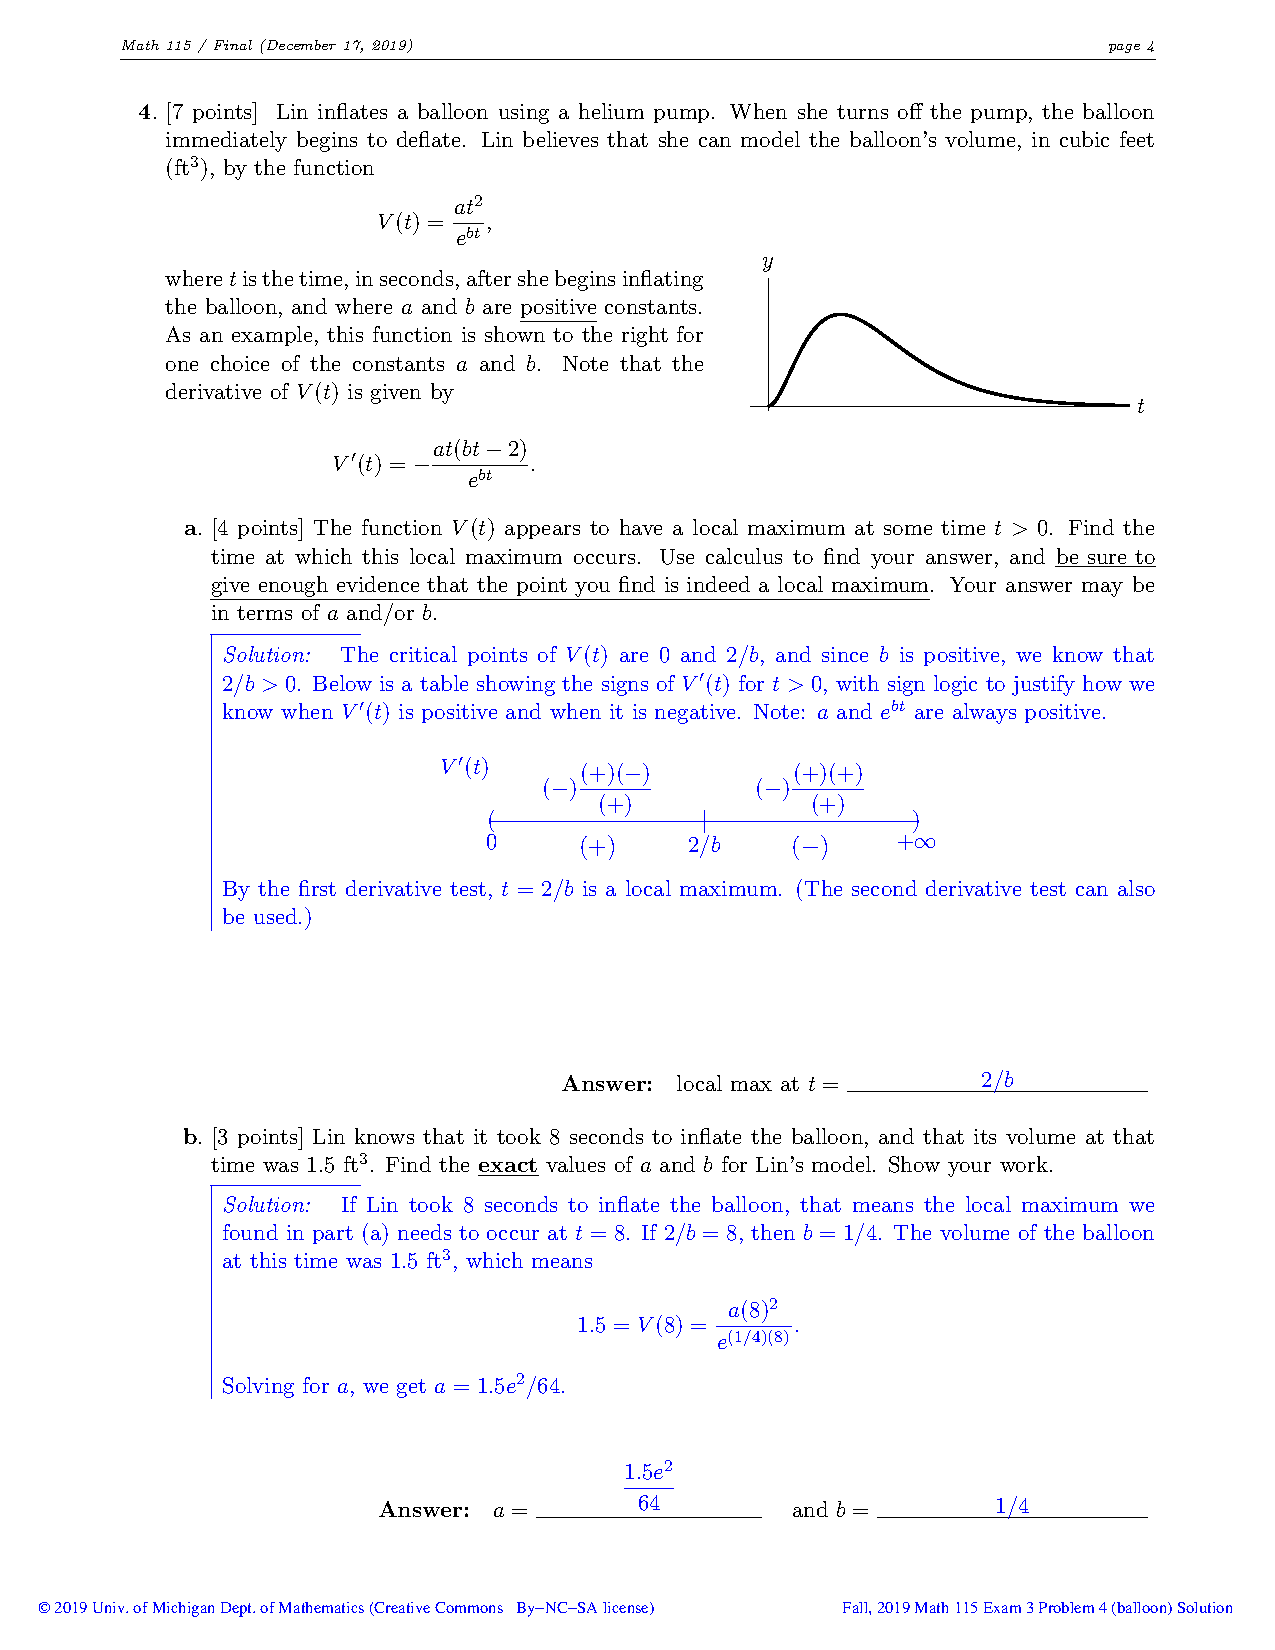
\includepdf[pages=-,pagecommand={}]{s4.pdf}
    \else
    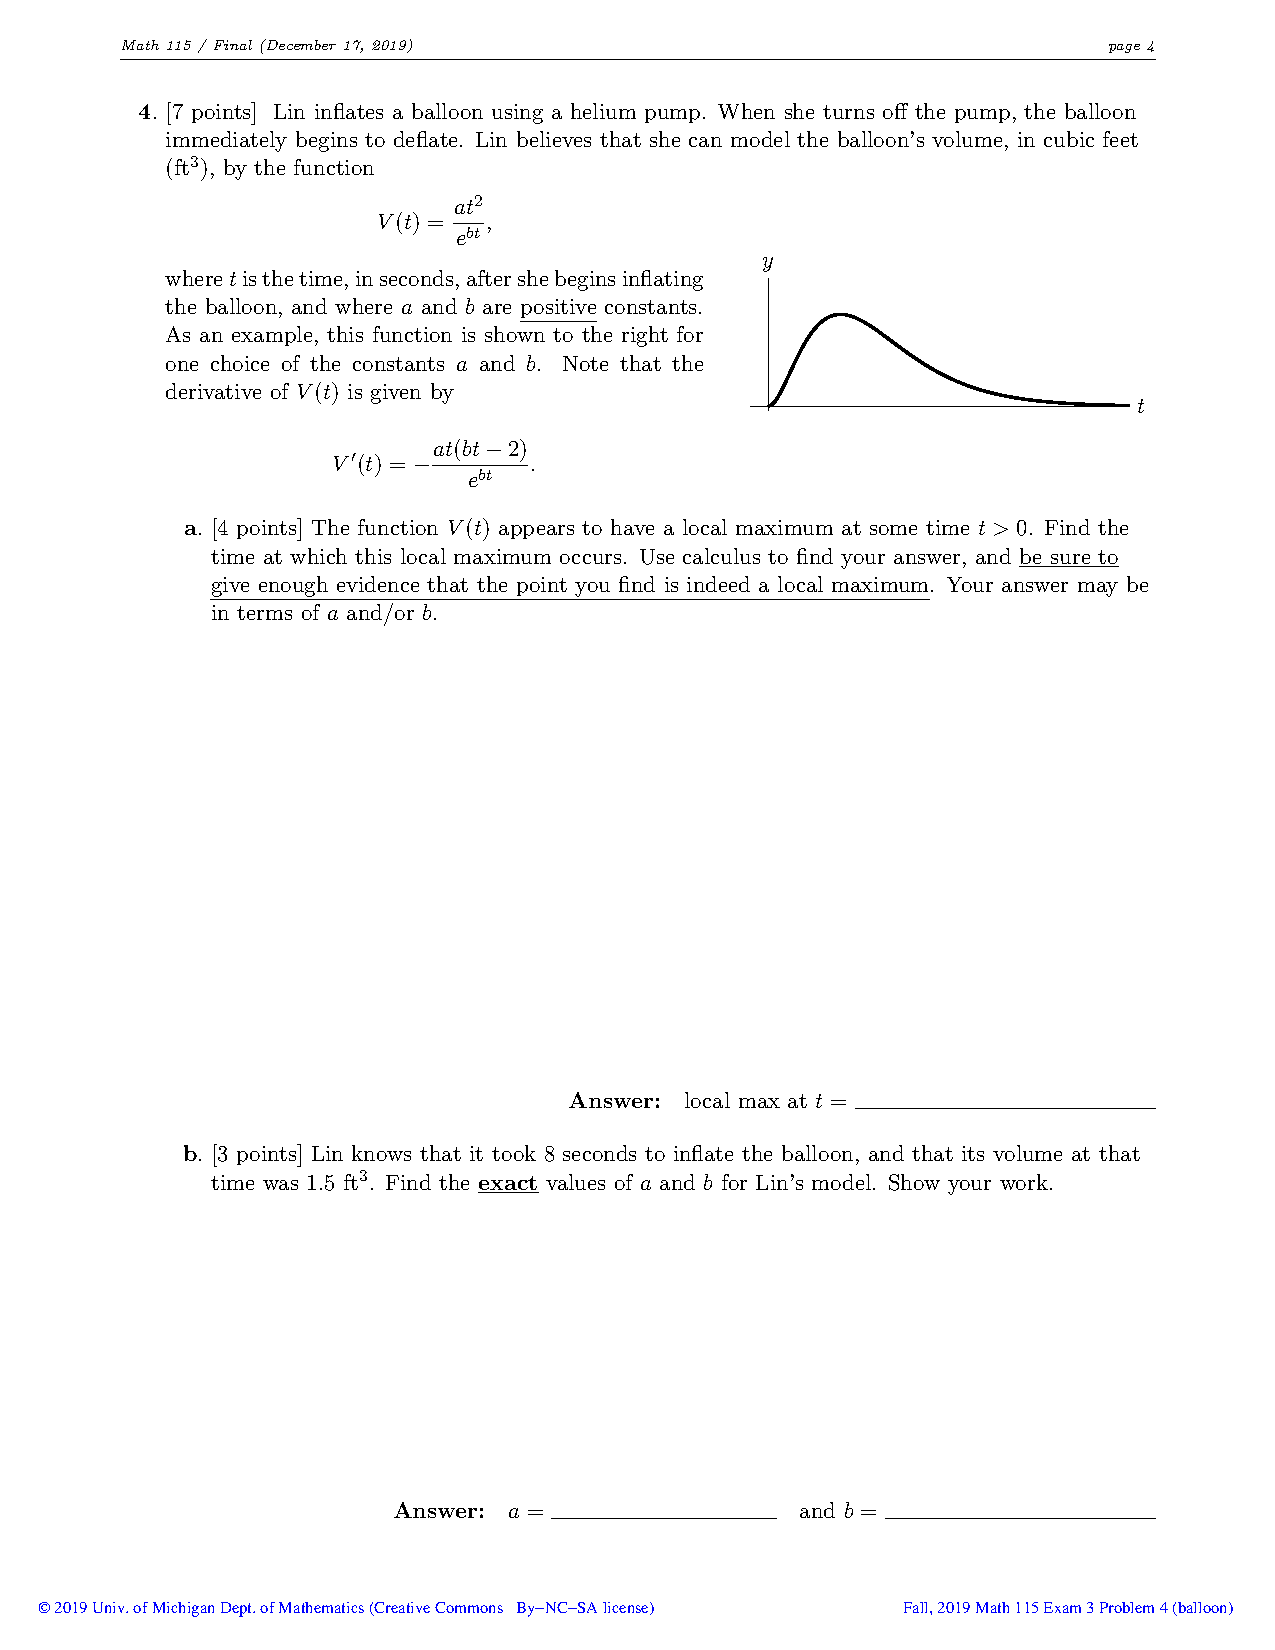
\includepdf[pages=-,pagecommand={}]{p4.pdf}
    \fi
    \pagebreak
    \pagebreak
    \ifprintanswers 
    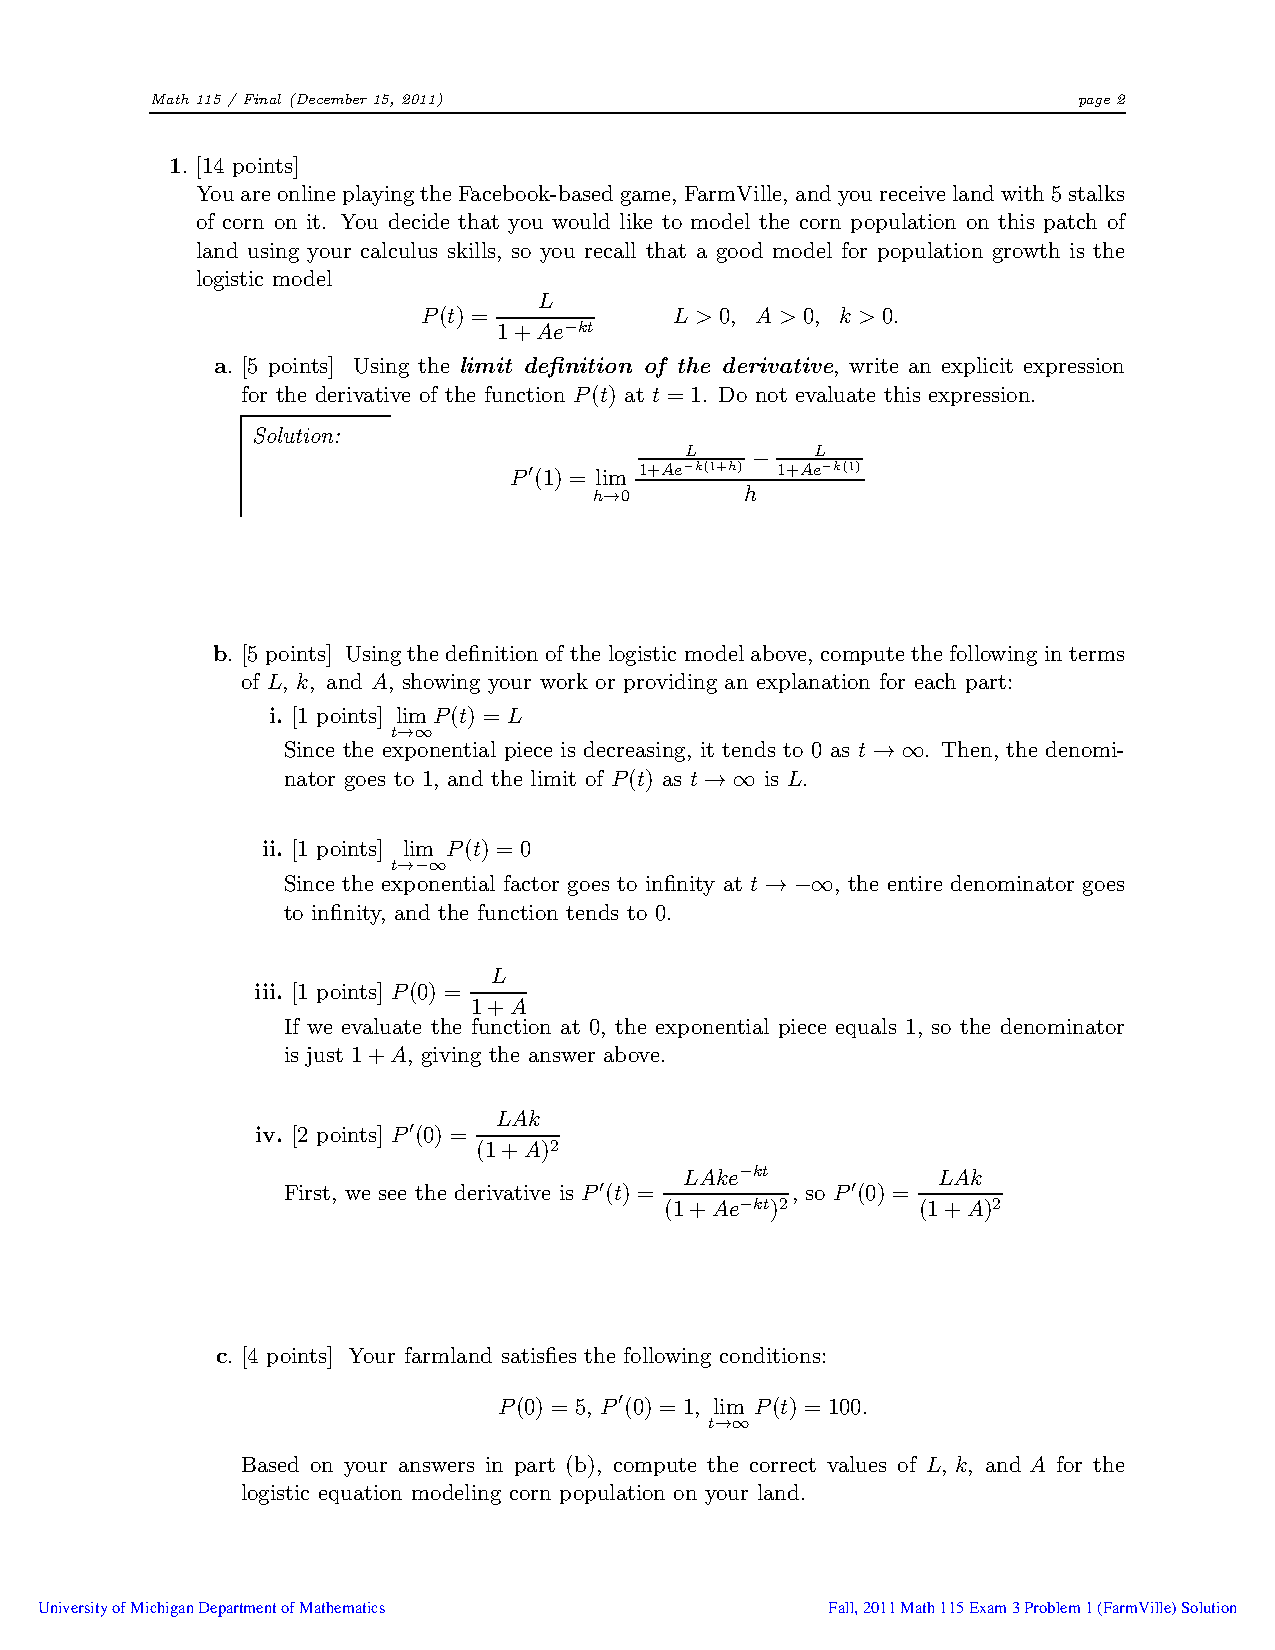
\includepdf[pages=-,pagecommand={}]{s1.pdf}
    \else
    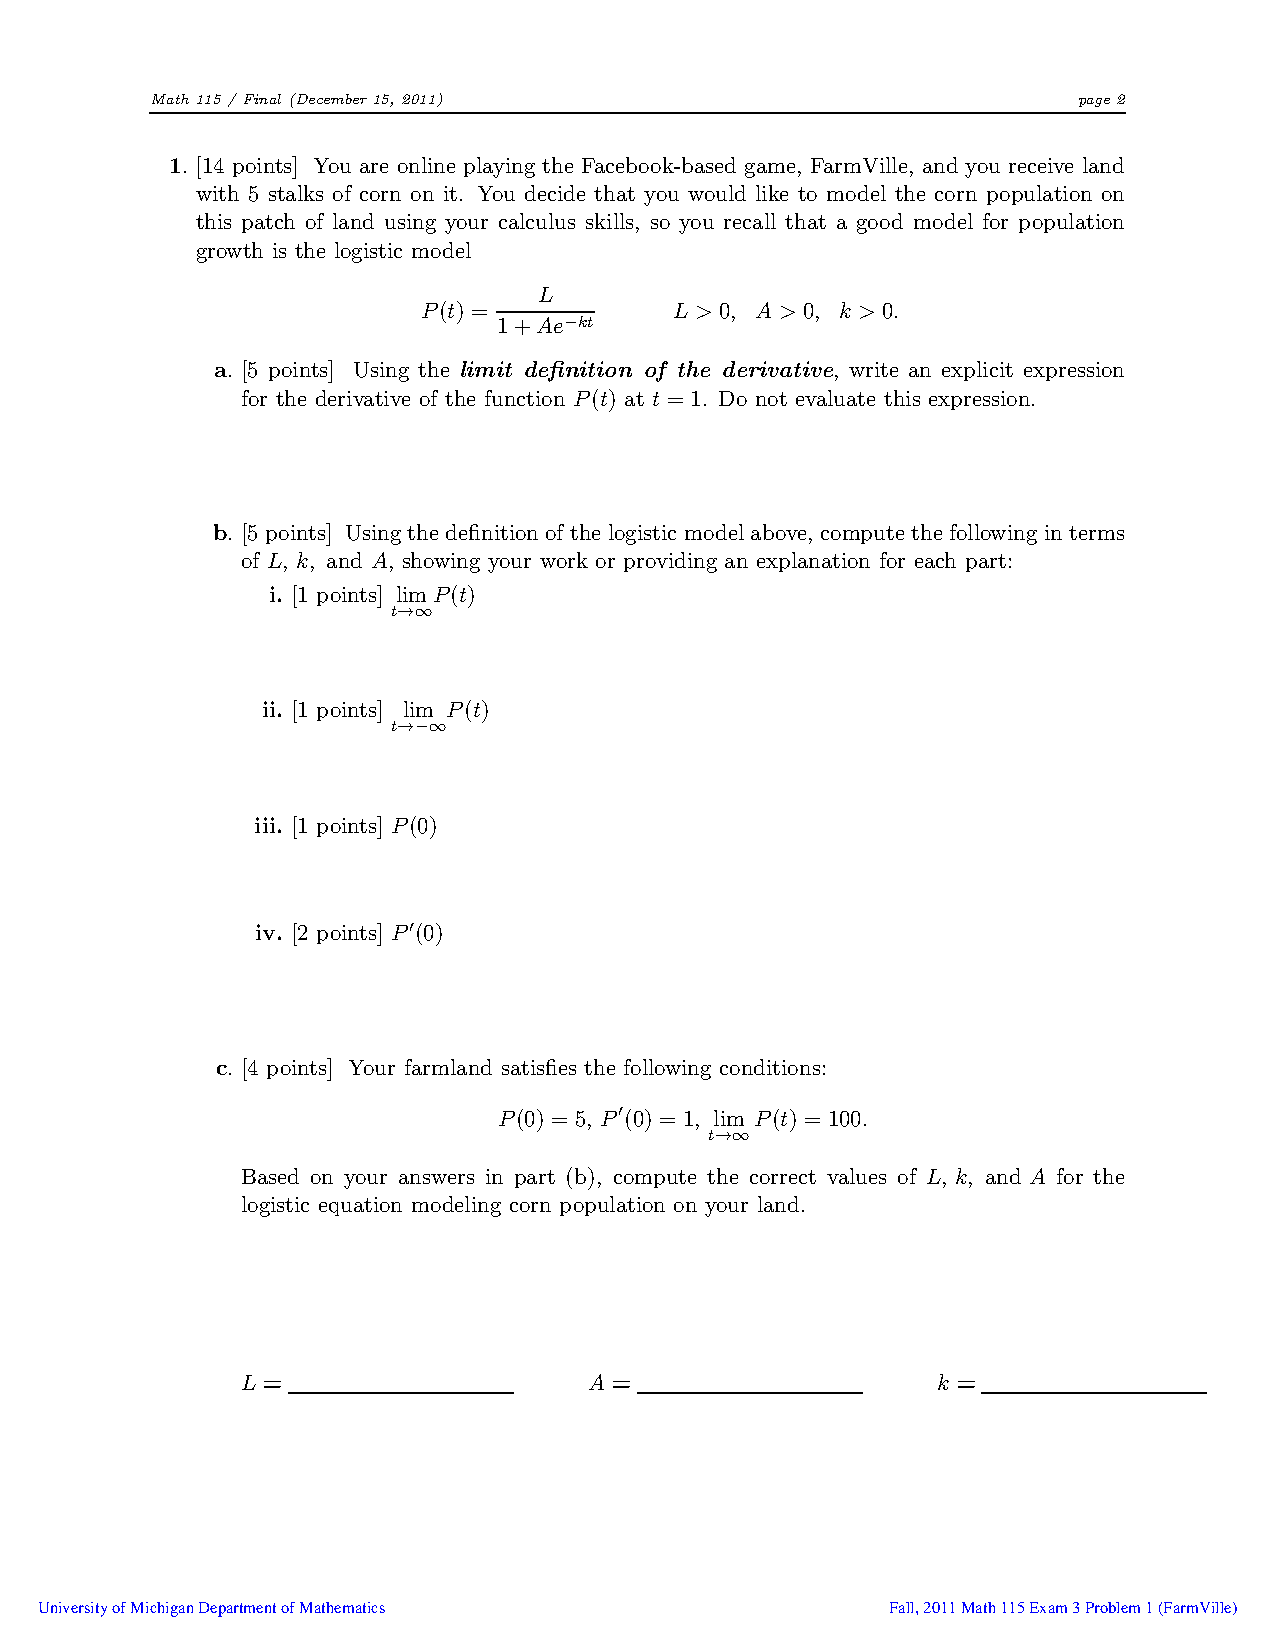
\includepdf[pages=-,pagecommand={}]{p1.pdf}
    \fi
    \pagebreak
    \pagebreak
    \ifprintanswers 
    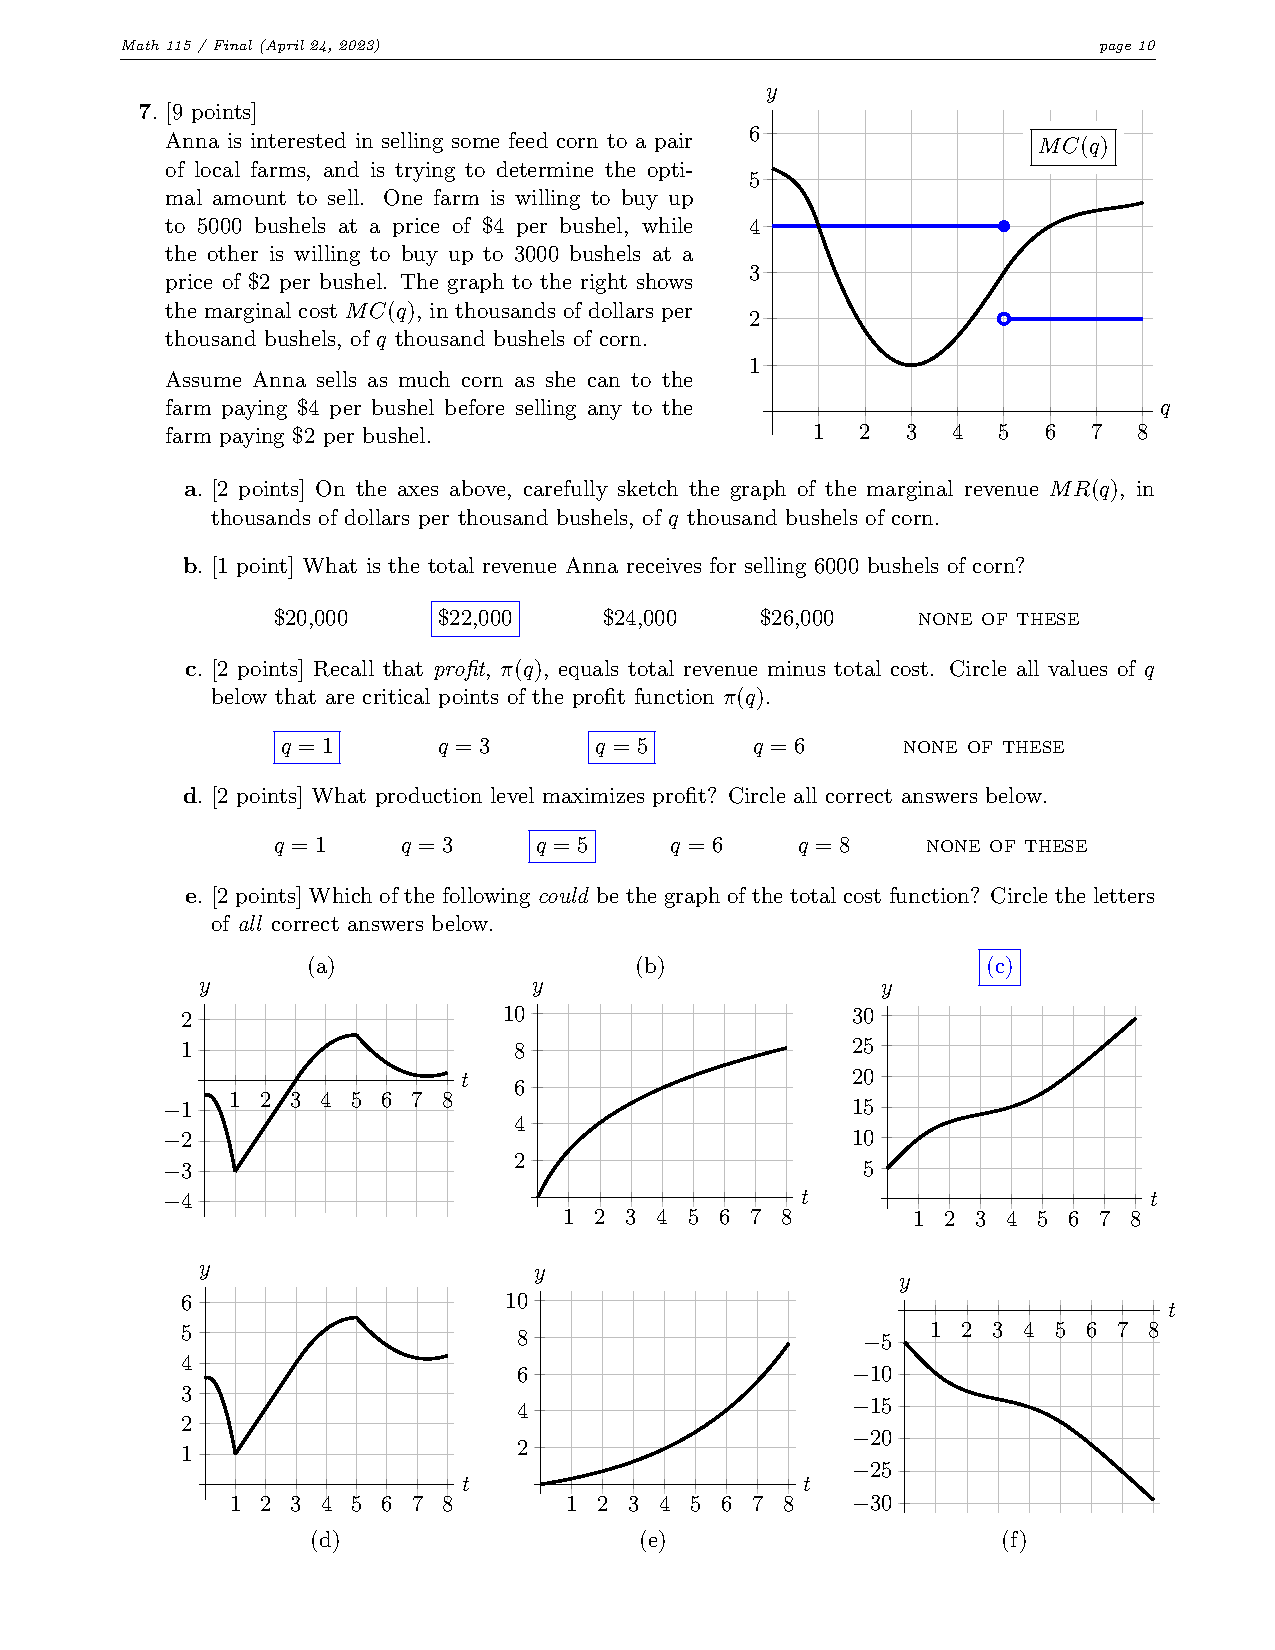
\includepdf[pages=-,pagecommand={}]{s7.pdf}
    \else
    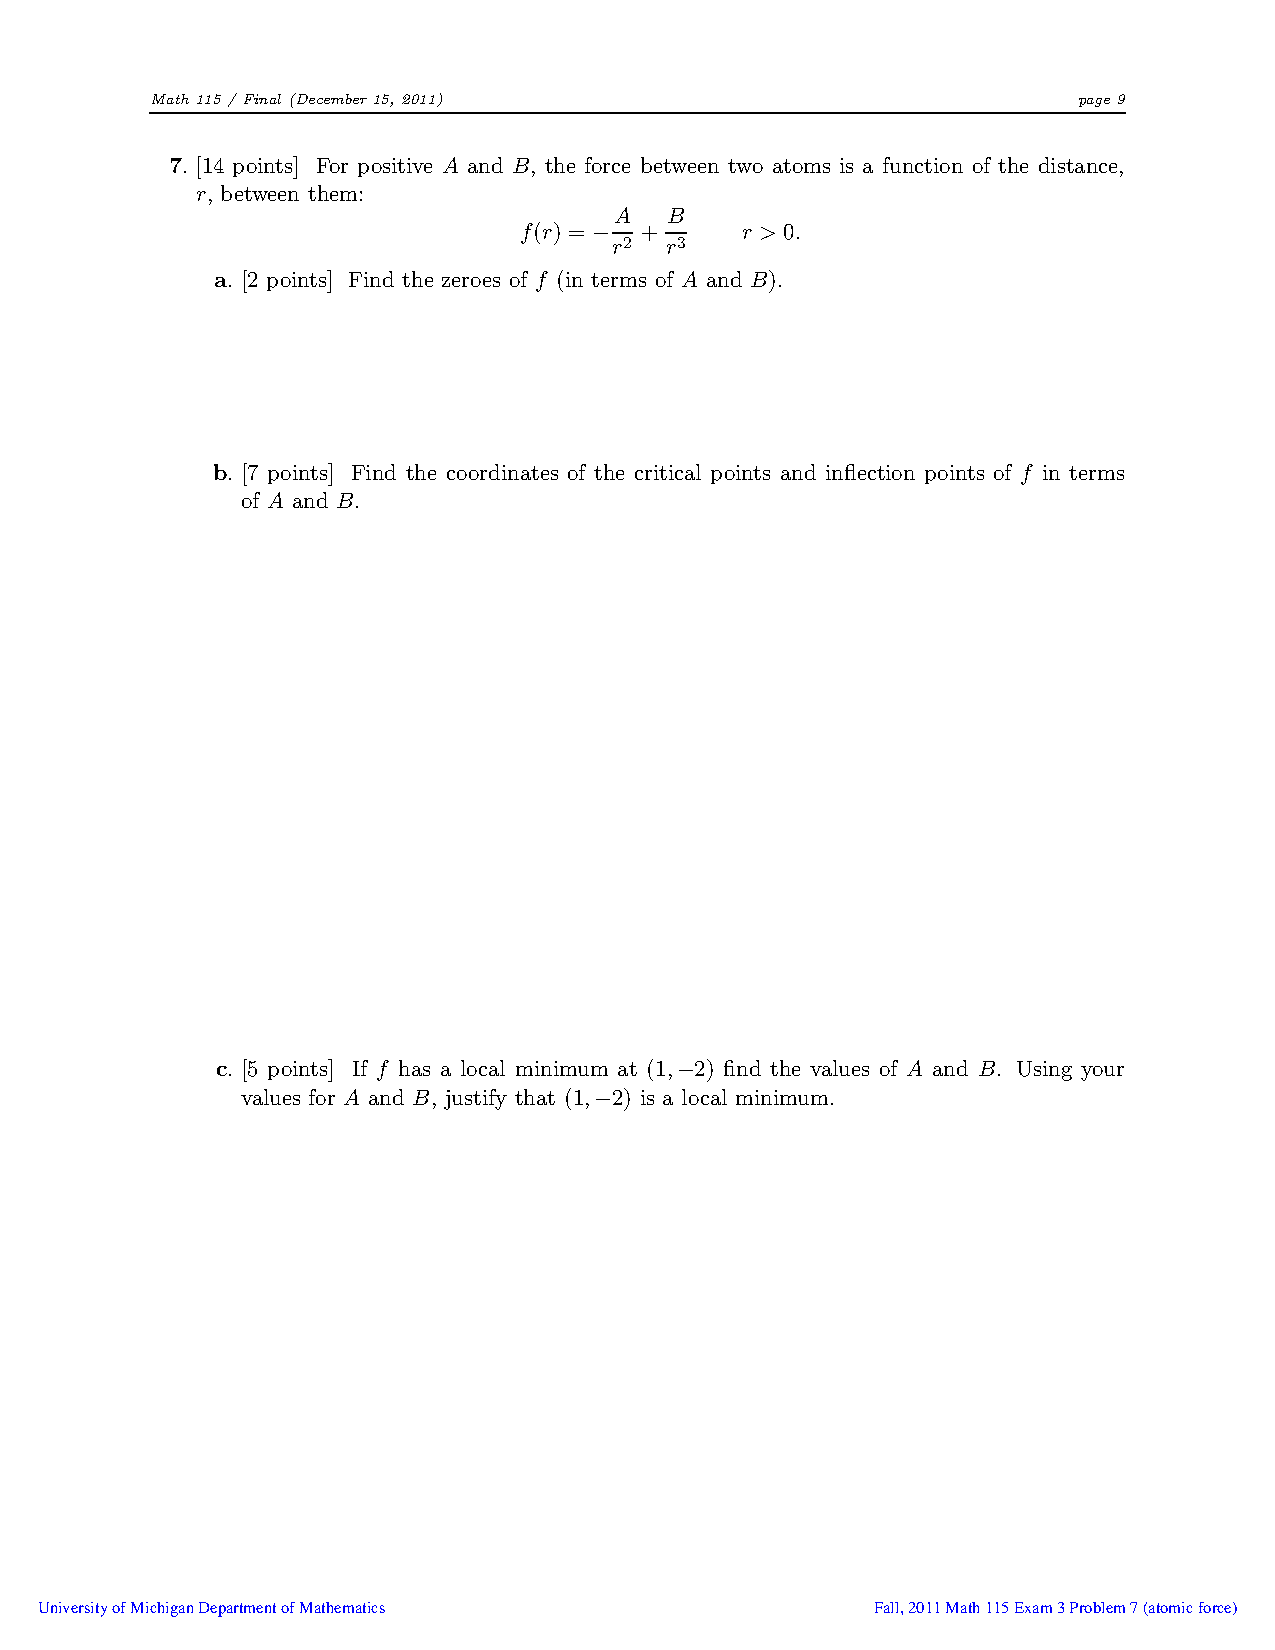
\includepdf[pages=-,pagecommand={}]{p7.pdf}
    \fi
    \pagebreak
    \pagebreak
    \ifprintanswers 
    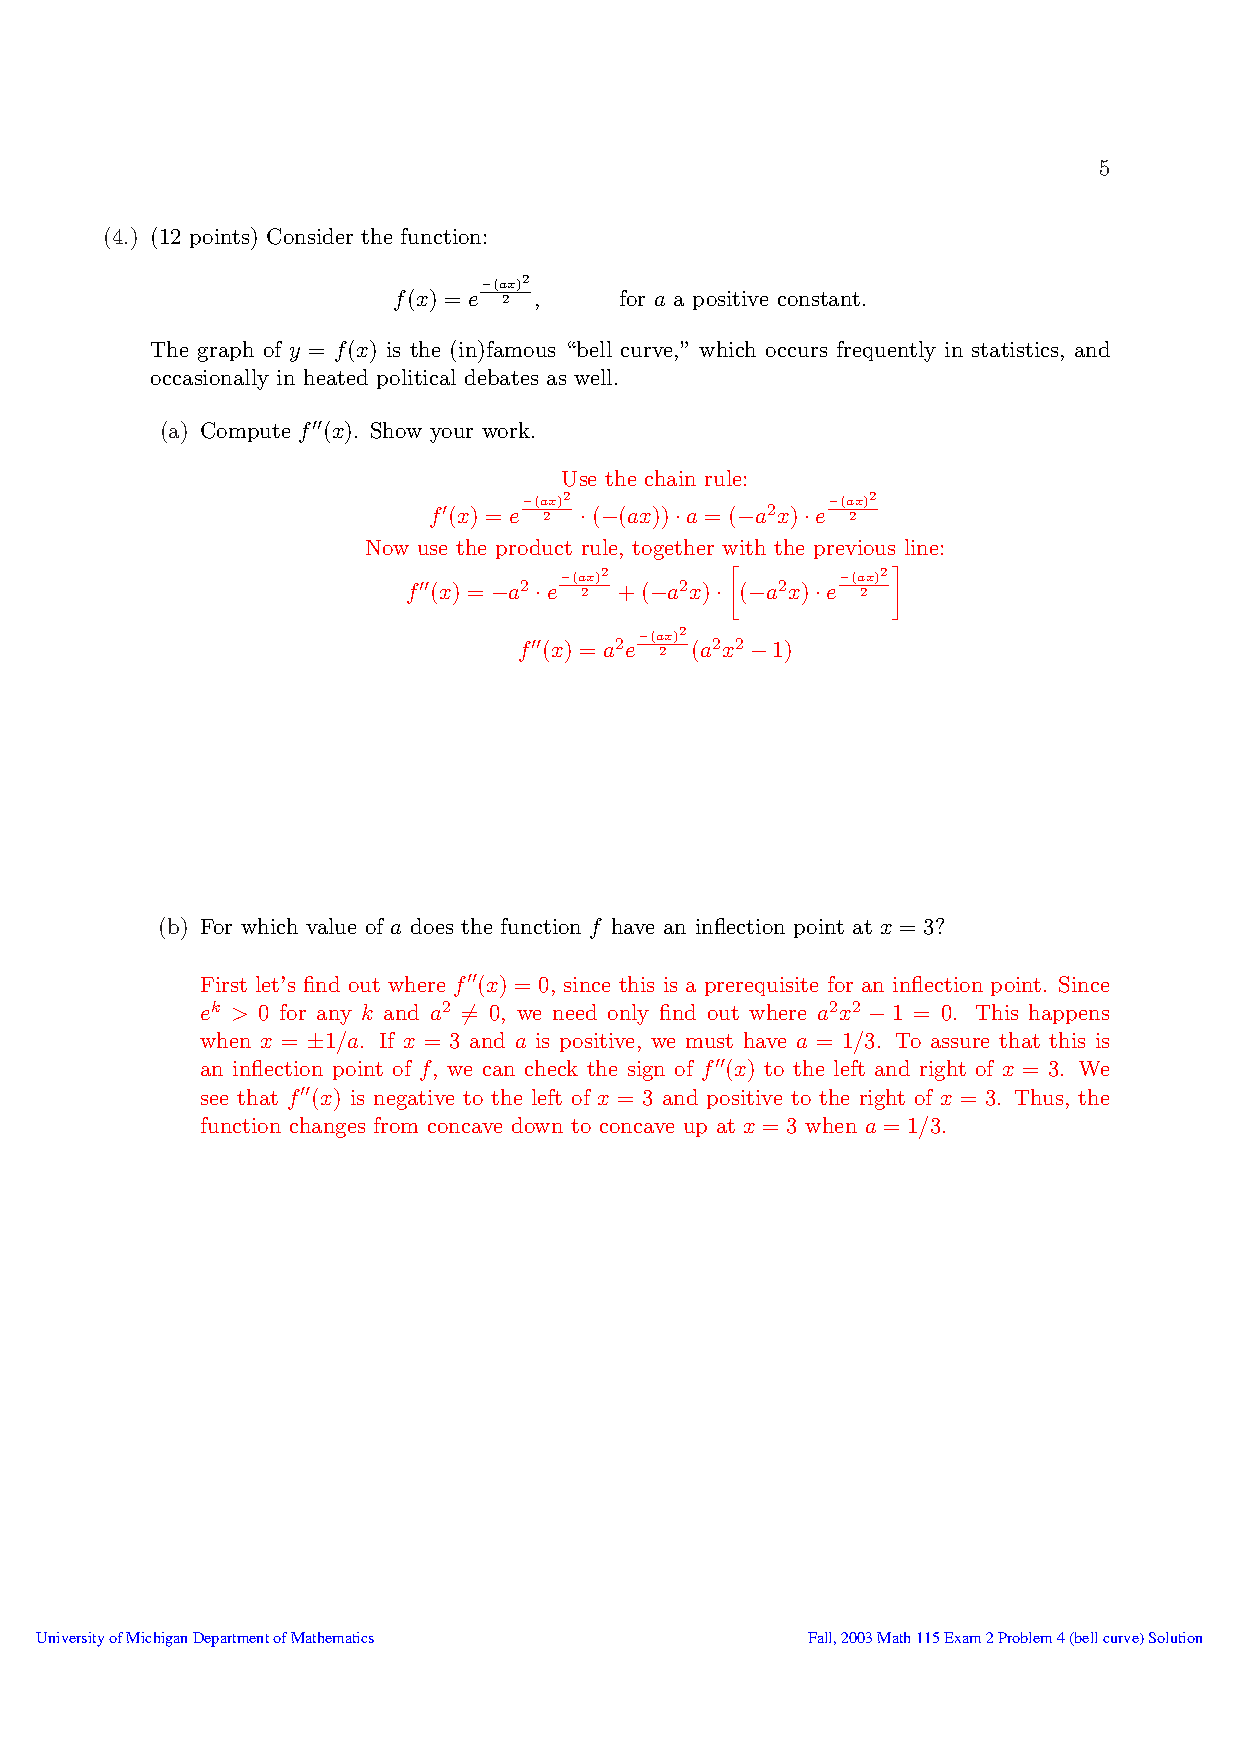
\includepdf[pages=-,pagecommand={}]{s4-2.pdf}
    \else
    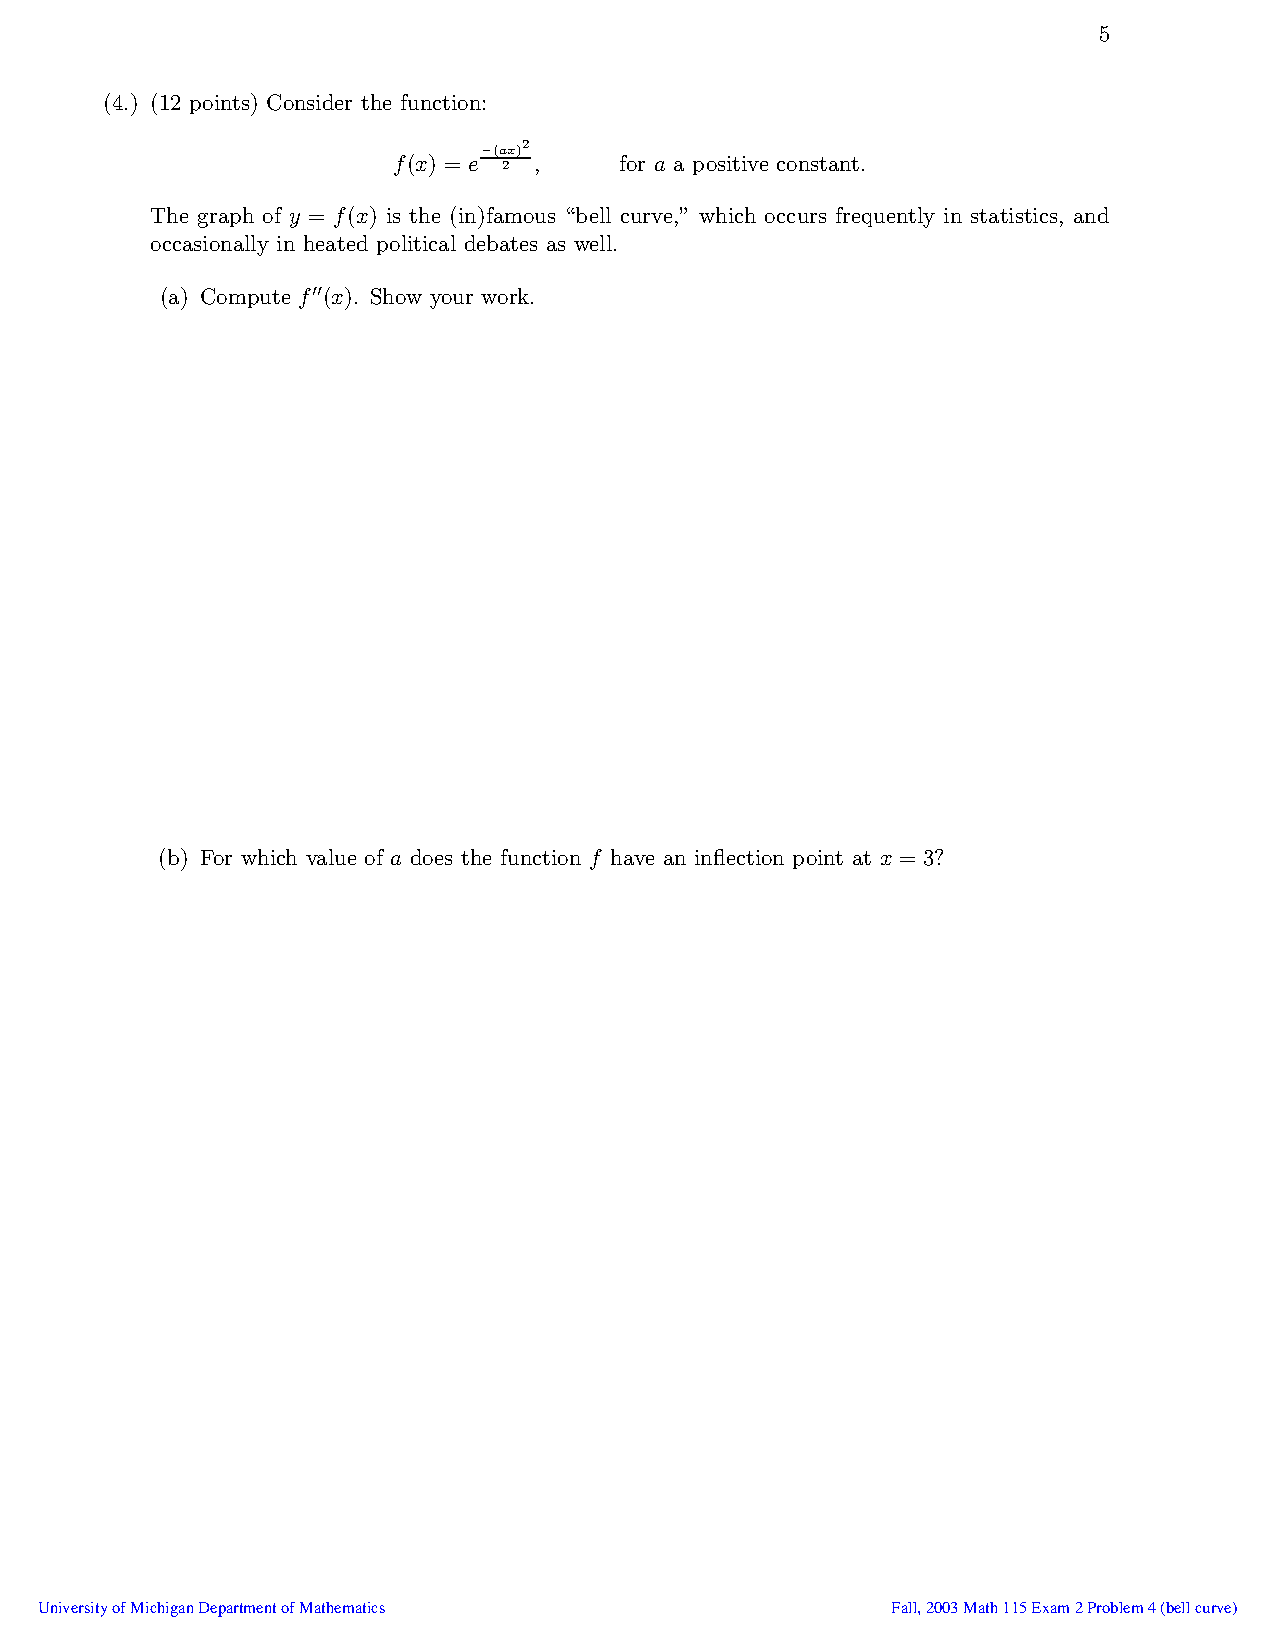
\includepdf[pages=-,pagecommand={}]{p4-2.pdf}
    \fi
    \pagebreak
    \pagebreak
    \ifprintanswers 
    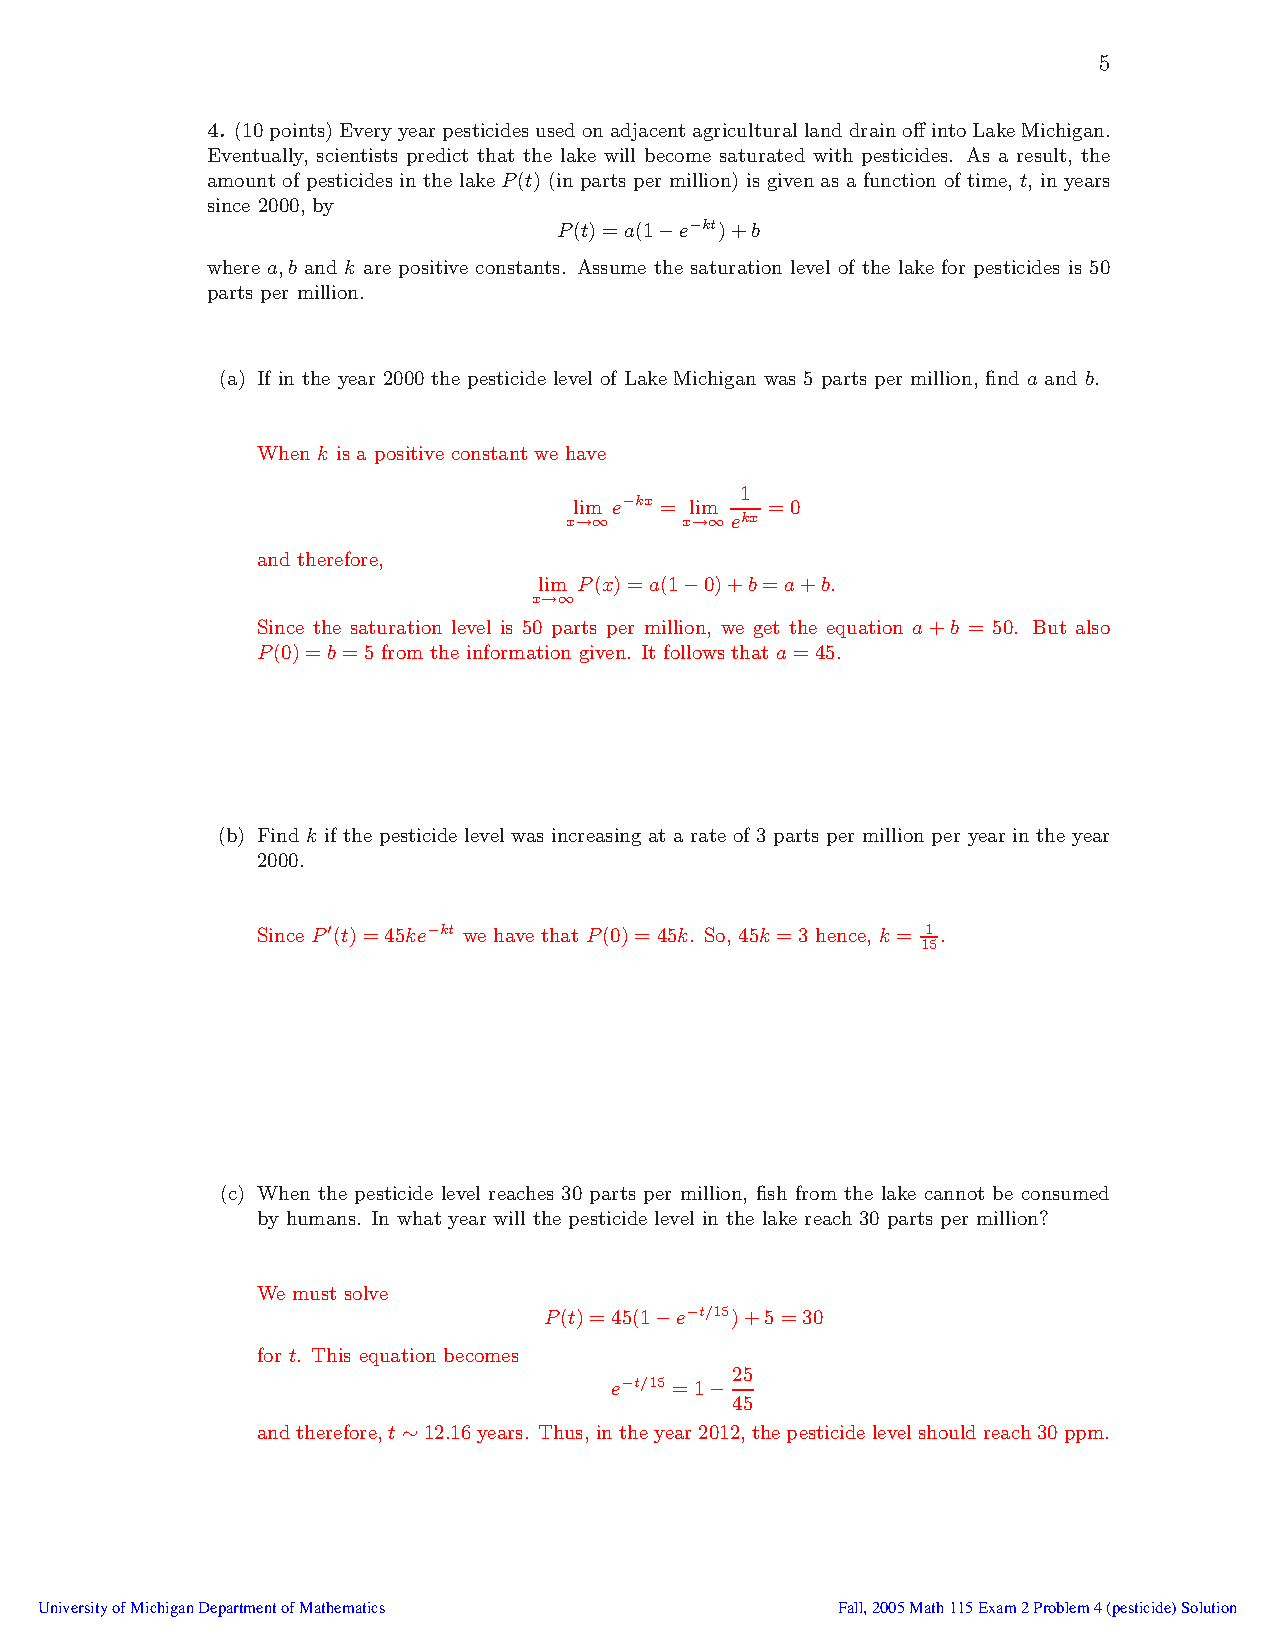
\includepdf[pages=-,pagecommand={}]{s4-3.pdf}
    \else
    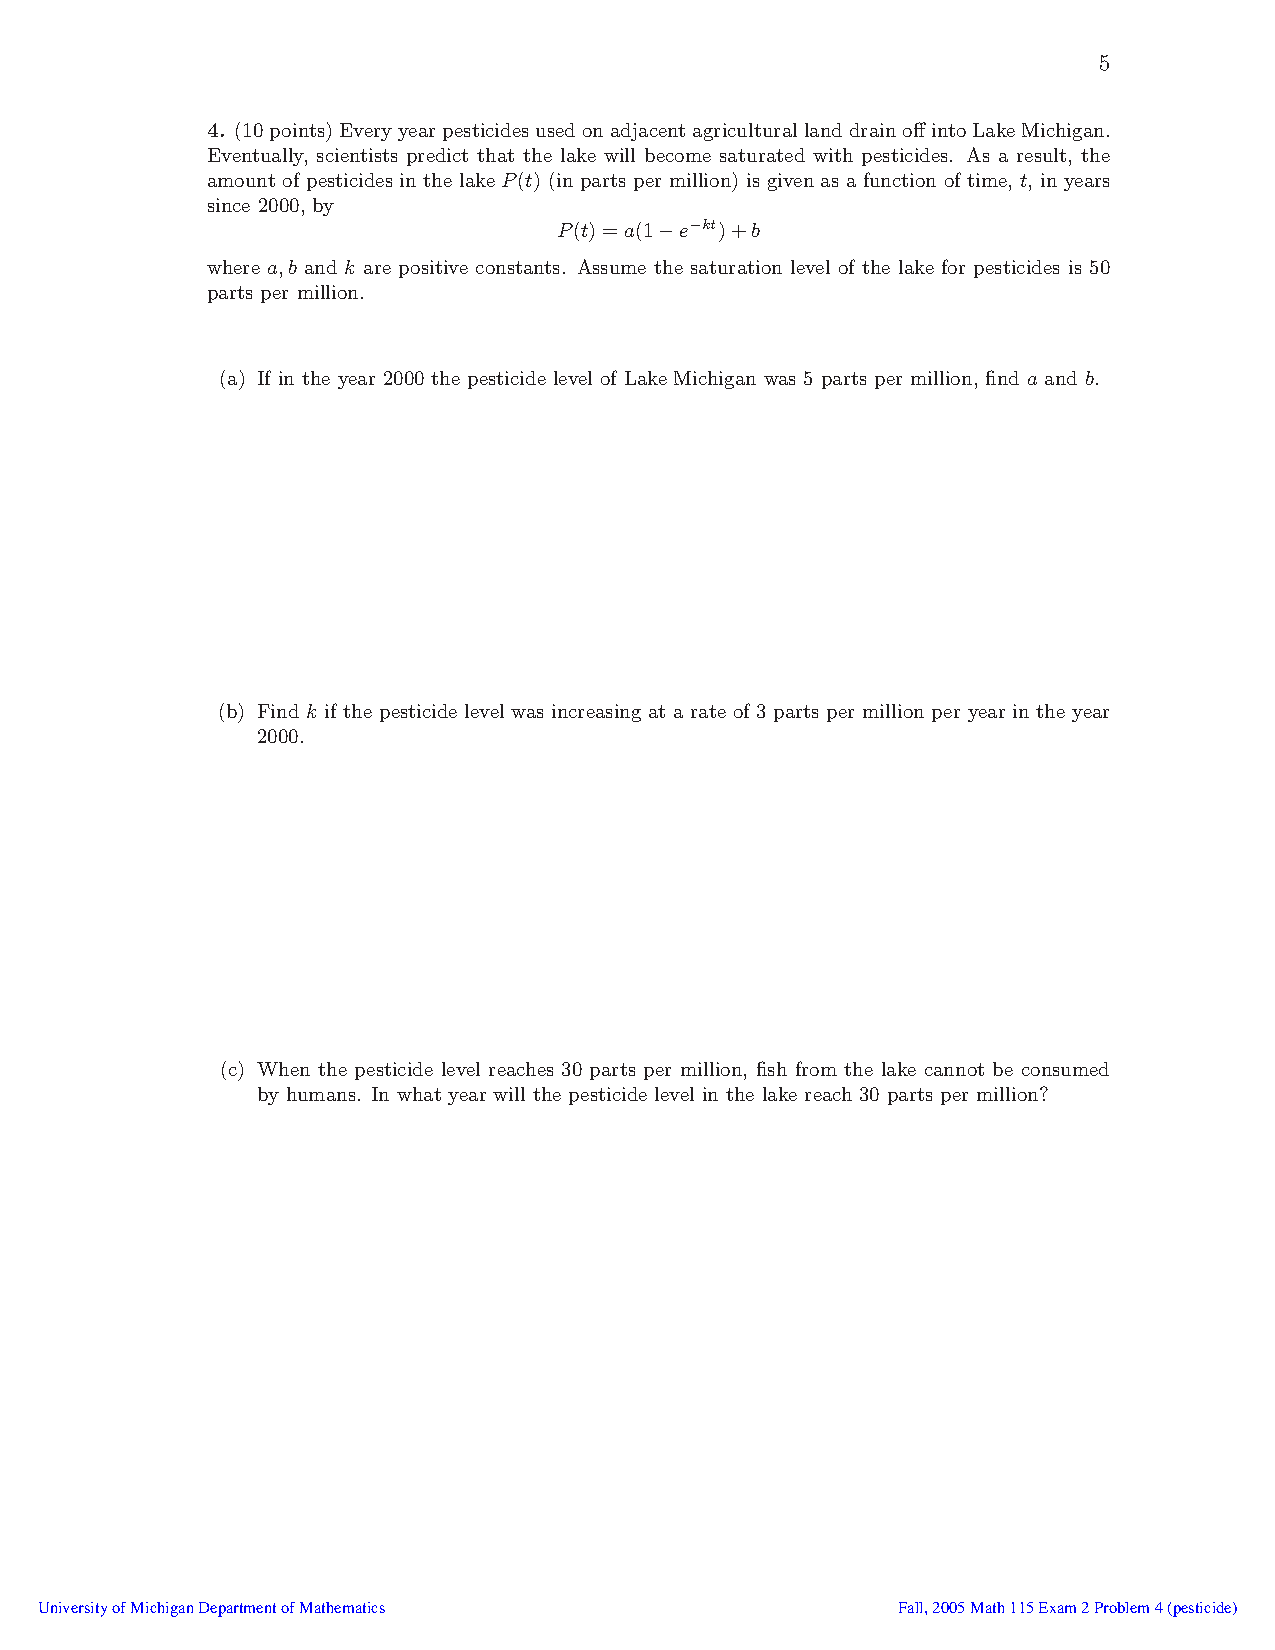
\includepdf[pages=-,pagecommand={}]{p4-3.pdf}
    \fi
\end{questions}
\end{document}
%%% Local Variables:
%%% mode: latex
%%% TeX-master: t
%%% End:
